\documentclass[compress,red]{beamer}
\usepackage[utf8]{inputenc}
\usepackage{ucs}
\usepackage{amsmath}
\usepackage{amsfonts}
\usepackage{amssymb}
\usepackage[russian]{babel}
\usepackage{graphicx}
\usepackage{wrapfig}

\usepackage{tikz}
\usepackage{verbatim}

\usepackage{color}
\usepackage{xcolor}
\usepackage{listings}

\usepackage{caption}

\lstset{
language=ruby,
extendedchars=\true,
inputencoding=utf8x,
commentstyle=\itshape,
stringstyle=\bf,
belowcaptionskip=5pt }


\DeclareCaptionFont{white}{\color{white}}
\DeclareCaptionFormat{listing}{\colorbox{gray}{\parbox{\textwidth}{#1#2#3}}}
\captionsetup[lstlisting]{format=listing,labelfont=white,textfont=white}

\usetikzlibrary{calc,trees,positioning,arrows,chains,shapes.geometric,%
    decorations.pathreplacing,decorations.pathmorphing,shapes,%
    matrix,shapes.symbols}

\tikzset{
>=stealth',
  punktchain/.style={
    rectangle, 
    rounded corners, 
    % fill=black!10,
    draw=black, very thick,
    text width=10em, 
    minimum height=3em, 
    text centered, 
    on chain},
  line/.style={draw, thick, <-},
  element/.style={
    tape,
    top color=white,
    bottom color=blue!50!black!60!,
    minimum width=8em,
    draw=blue!40!black!90, very thick,
    text width=10em, 
    minimum height=1.5em, 
    text centered, 
    on chain},
  every join/.style={->, thick,shorten <=1pt},
  decoration={brace},
  tuborg/.style={decorate},
  tubnode/.style={midway, right=2pt},
}

\mode<presentation>

\usetheme{Warsaw}

\definecolor{Red}{rgb}{1,0,0}
\definecolor{Blue}{rgb}{0,0,1}
\definecolor{Green}{rgb}{0,1,0}
\definecolor{magenta}{rgb}{1,0,.6}
\definecolor{lightblue}{rgb}{0,.5,1}
\definecolor{lightpurple}{rgb}{.6,.4,1}
\definecolor{gold}{rgb}{.6,.5,0}
\definecolor{orange}{rgb}{1,0.4,0}
\definecolor{hotpink}{rgb}{1,0,0.5}
\definecolor{newcolor2}{rgb}{.5,.3,.5}
\definecolor{newcolor}{rgb}{0,.3,1}
\definecolor{newcolor3}{rgb}{1,0,.35}
\definecolor{darkgreen1}{rgb}{0, .35, 0}
\definecolor{darkgreen}{rgb}{0, .6, 0}
\definecolor{darkred}{rgb}{.75,0,0}

\xdefinecolor{olive}{cmyk}{0.64,0,0.95,0.4}
\xdefinecolor{purpleish}{cmyk}{0.75,0.75,0,0}

\useoutertheme[subsection=false]{smoothbars}

\title{Блогосфера}
\author{Информатика \\ 10-11 классы}

%\usecolortheme{dolphin}


\begin{document}
%%титульная страница
\maketitle
%% основные моменты

\section{Блогосфера}

\subsection{Блогосфера}
\begin{frame}
  \frametitle{Блогосфера}
	\centerline{
\includegraphics[width=0.8\textwidth]{images/blogosphere.png}}
\end{frame}

\subsection{Определение}
\begin{frame}[fragile]
\frametitle{Что это такое?}
		\begin{itemize}
		\item Под термином \emph{блогосфера} обычно понимают совокупность всех блогов как сообщество.
		\item Более корректно так: блогосфера = блоги + микроблоги + социальные сети.
		\item Микроблог --- это блог с ограничениями по длине сообщений. Пример: Twitter (http://twitter.com)
		\item Помимо Blogger'а от Google существует множество других платформ для ведения блогов: Livejournal, MySpace, Я.ру, Diary и др..
		\end{itemize}
\end{frame}

\subsection{Livejournal}
\begin{frame}
  \frametitle{Livejournal}
	\centerline{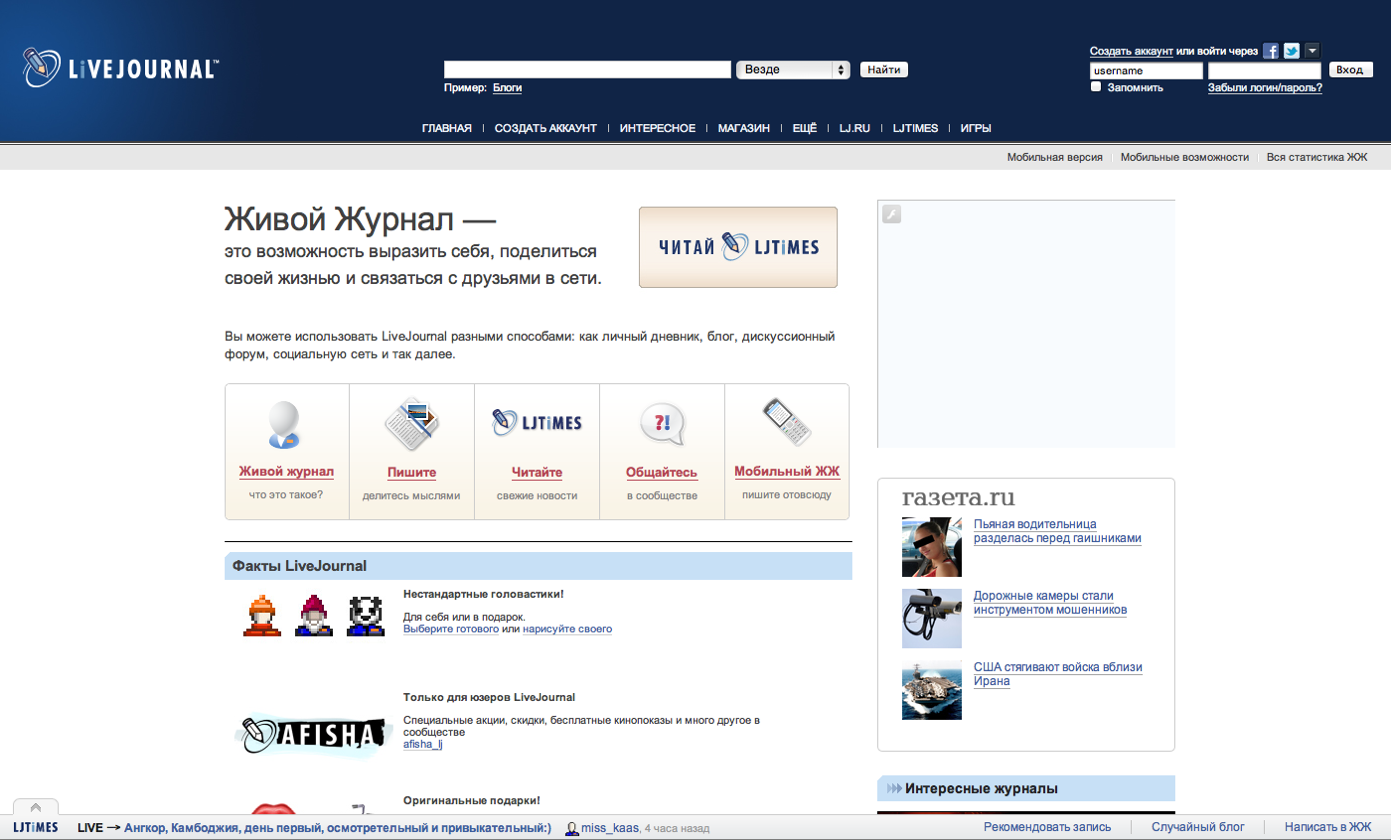
\includegraphics[width=0.8\textwidth]{images/livejournal.png}}
\end{frame}

\subsection{Описание}
\begin{frame}[fragile]
\frametitle{Livejournal: описание}
		\begin{itemize}
		\item Livejournal или Живой журнал. Сленговое название: ЖЖ, жежешечка.
		\item Самый популярный сервис ведения блогов в России.
		\item Все популярные люди, имеющие свой блог, имеют как минимум его ``клон'' в ЖЖ.
		\item Основная ``фишка'' сервиса --- лента друзей (\emph{френдлента}). В ней находятся обновления всех пользователей, которых вы добавили в друзья.
		\item Также интересен следующий дополнительный функционал: настройка приватности (сообщение только для себя / друзей / всех), настройка аватаров (юзерпиков) для каждого поста, сообщества.
		\end{itemize}
\end{frame}

\subsection{Livejournal: примеры}
\begin{frame}
  \frametitle{Livejournal: примеры}
	\centerline{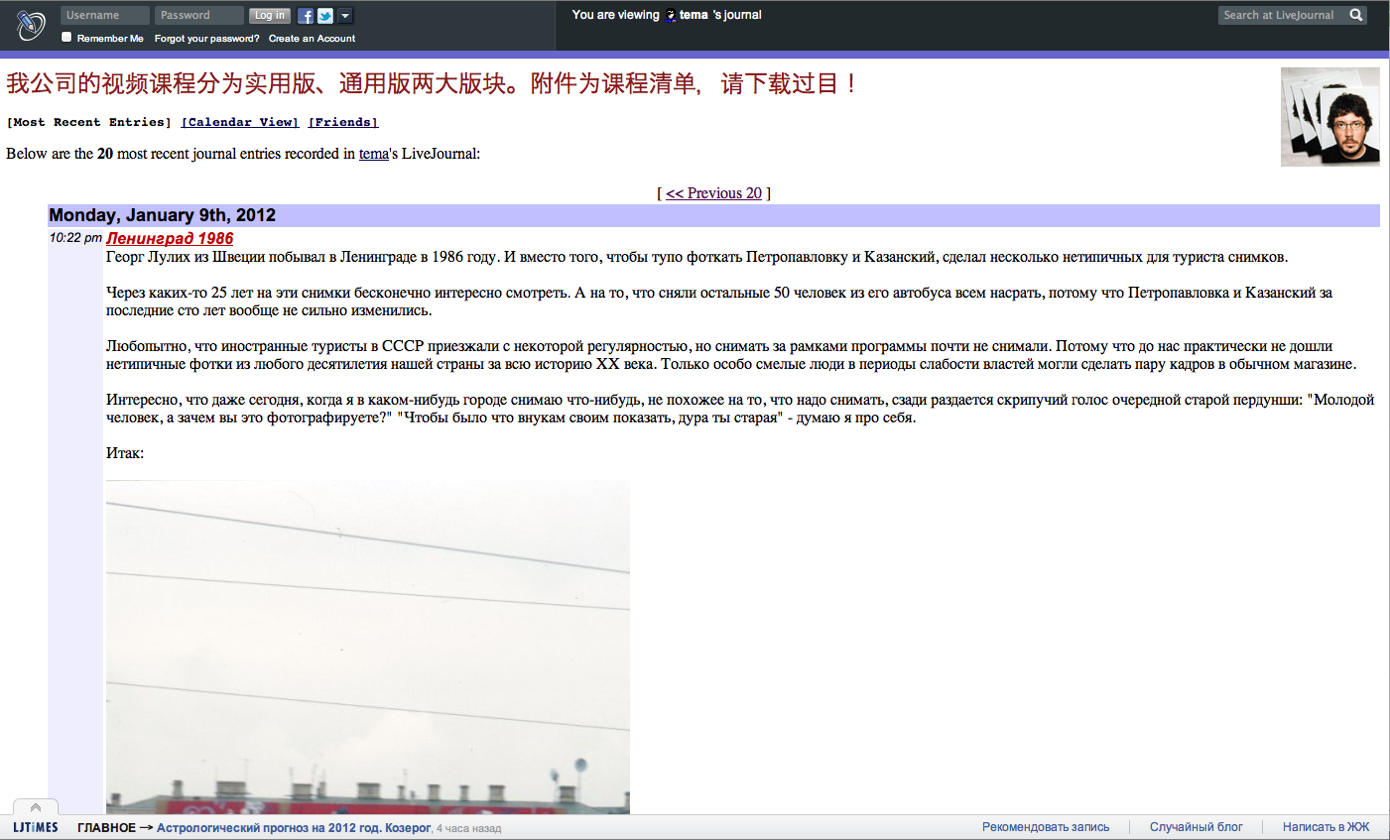
\includegraphics[width=0.8\textwidth]{images/tema-lj.png}}
\end{frame}

\subsection{Livejournal: примеры}
\begin{frame}
  \frametitle{Livejournal: примеры}
	\centerline{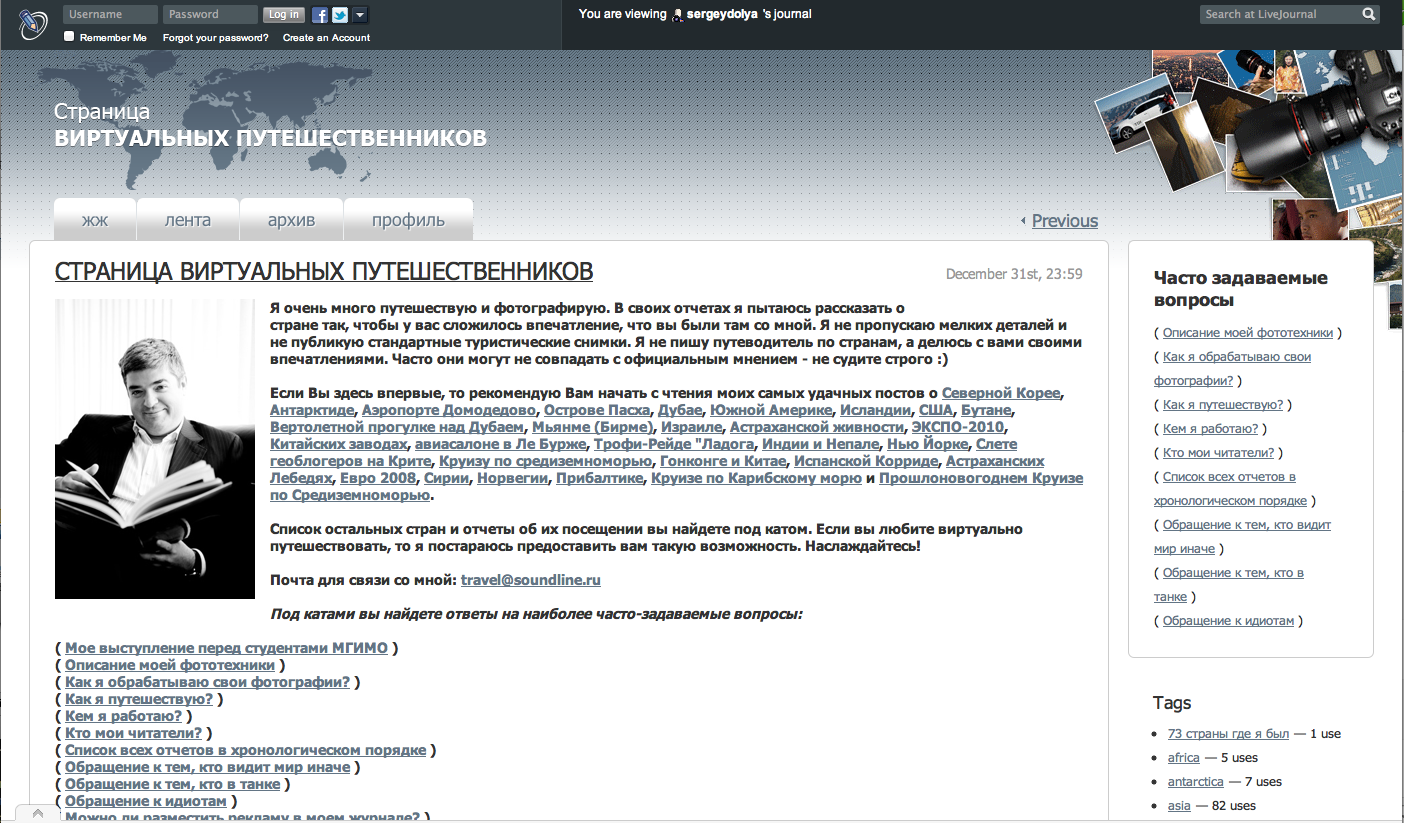
\includegraphics[width=0.8\textwidth]{images/sergeydolya-lj.png}}
\end{frame}

\section{Twitter}
\subsection{Twitter}
\begin{frame}
  \frametitle{Twitter}
	\centerline{
\includegraphics[width=0.8\textwidth]{images/twitter.png}}
\end{frame}

\subsection{Видеообзор}
\begin{frame}
  \frametitle{Видеообзор}
	\begin{itemize}
	\item http://www.youtube.com/watch?v=ddO9idmax0o
	\item http://goo.gl/qGWlV (субтитры)
	\end{itemize}
\end{frame}

\subsection{Основные возможности}
\begin{frame}
  \frametitle{Основные возможности}
	\begin{itemize}
	\item Публикация коротких сообщений до 140 символов.
	\item Разные типы сообщений: 
		\begin{enumerate}
			\item твит (что делаю или о чём думаю),
			\item ответ на чей-то статус,
			\item ретвит (повтор чужого статуса),
			\item фото (с комментарием опционально),
			\item видео,
			\item ссылка на что-то интересное.
		\end{enumerate}
	\item Подписка (фоллов) на публичные аккаунты, списки читателей.
	\item Поиск по хэштегу (о каком-то событие. К примеру \#рождество)
	\end{itemize}
\end{frame}

\subsection{Сообщение}
\begin{frame}
	\begin{center}
	\large{vasya\_pupkin: Наши выиграли 3:1 http://goo.gl/8XTIq. У Бразилии. \#футбол \#победа}
	\end{center}
\end{frame}

\subsection{Сообщение}
\begin{frame}
	\begin{center}
	\large{petya\_nepupkin: @vasya\_pupkin В ФУТБОЛ??!!! \#футбол \#невероятно}
	\end{center}
\end{frame}

\subsection{Пример}
\begin{frame}
  \frametitle{Пример}
	\centerline{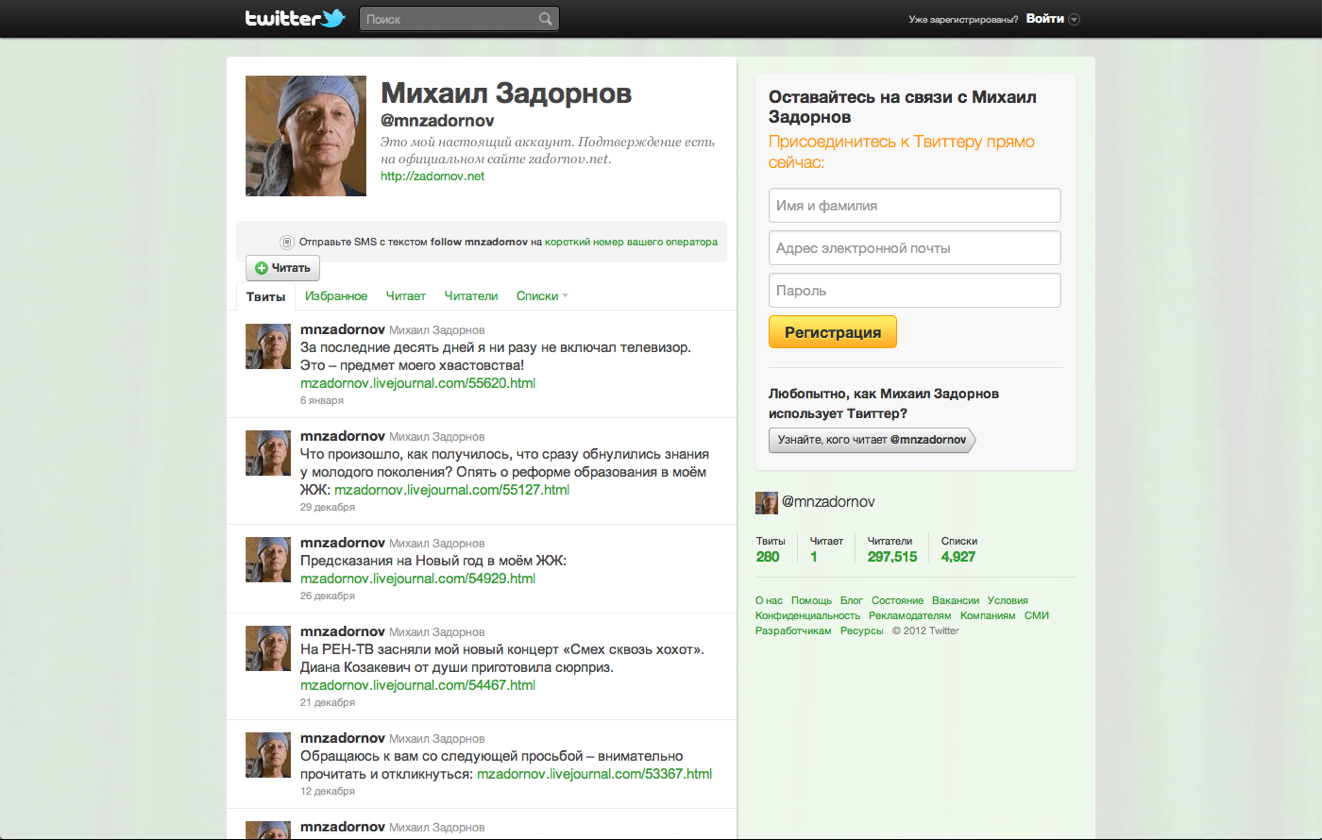
\includegraphics[width=0.9\textwidth]{images/twitter-mzadornov.png}}
\end{frame}

\section{Популярность блога}
\subsection{Популярность}
\begin{frame}
	\begin{center}
	\Huge{Как оценить популярность блога?}
	\end{center}
\end{frame}

\subsection{Популярность}
\begin{frame}
	\begin{center}
	\Large{Количество читателей?}
	\end{center}
\end{frame}

\subsection{Популярность}
\begin{frame}
	\begin{center}
	\Large{Количество просмотров?}
	\end{center}
\end{frame}

\subsection{Популярность}
\begin{frame}
	\begin{center}
	\Large{Количество комментариев?}
	\end{center}
\end{frame}

\subsection{Яндекс.Блоги}
\begin{frame}
  \frametitle{Яндекс.Блоги}
	\centerline{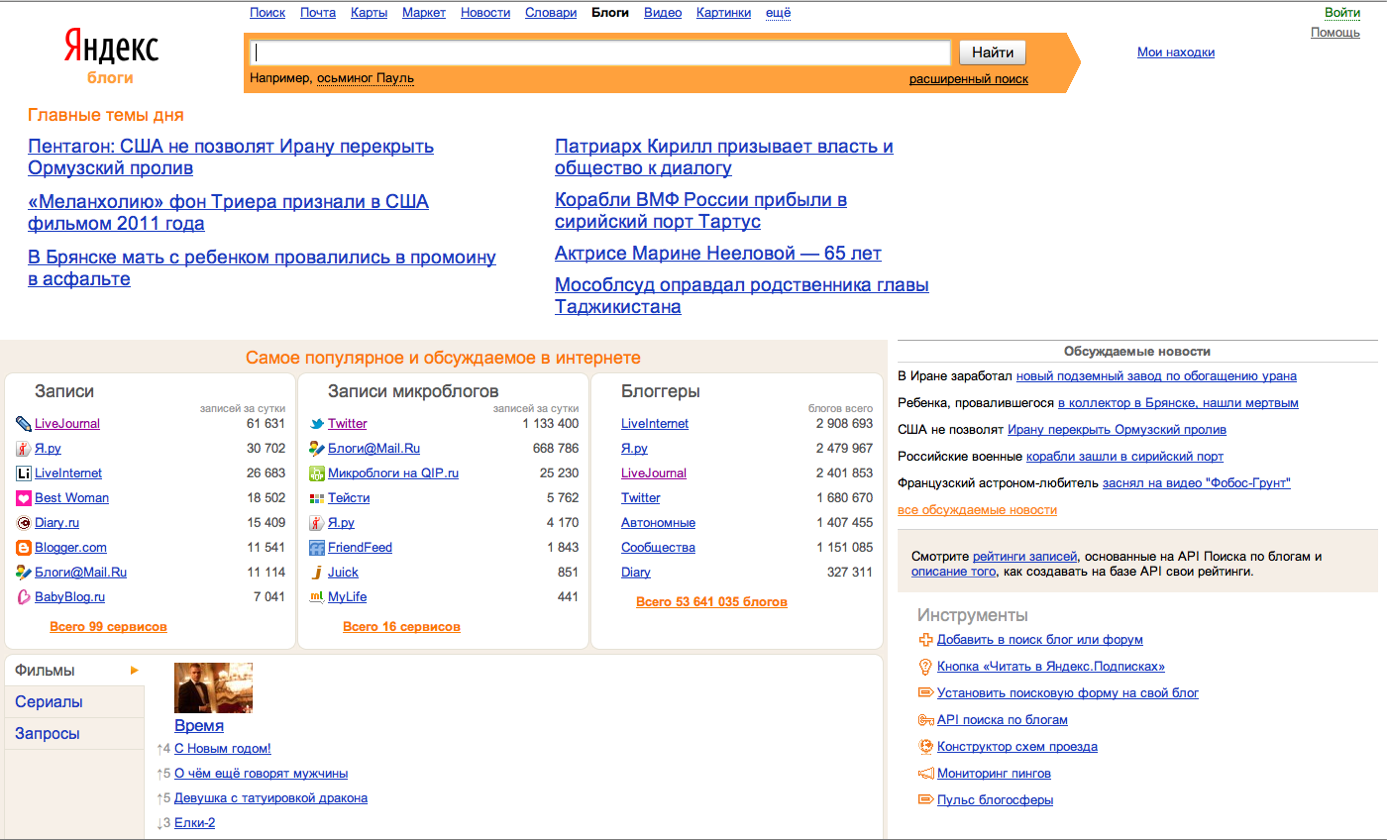
\includegraphics[width=0.9\textwidth]{images/blogs-yandex.png}}
\end{frame}

\subsection{Ответ}
\begin{frame}
  \frametitle{Яндекс.Блоги}
	\begin{itemize}
		\item Любой объективный параметр может использоваться.
		\item Яндексом для каждого блога (http://blogs.yandex.ru) оценивается \emph{авторитетность} --- интегральный рейтинг вышеуказанных свойств + ещё несколько.
		\item Для разных платформ рейтинг оценивается по разному.
		\item Рейтинг меняется со временем (КЭП).
	\end{itemize}
\end{frame}

\subsection{Яндекс.Боги}
\begin{frame}
  \frametitle{Яндекс.Боги}
	\centerline{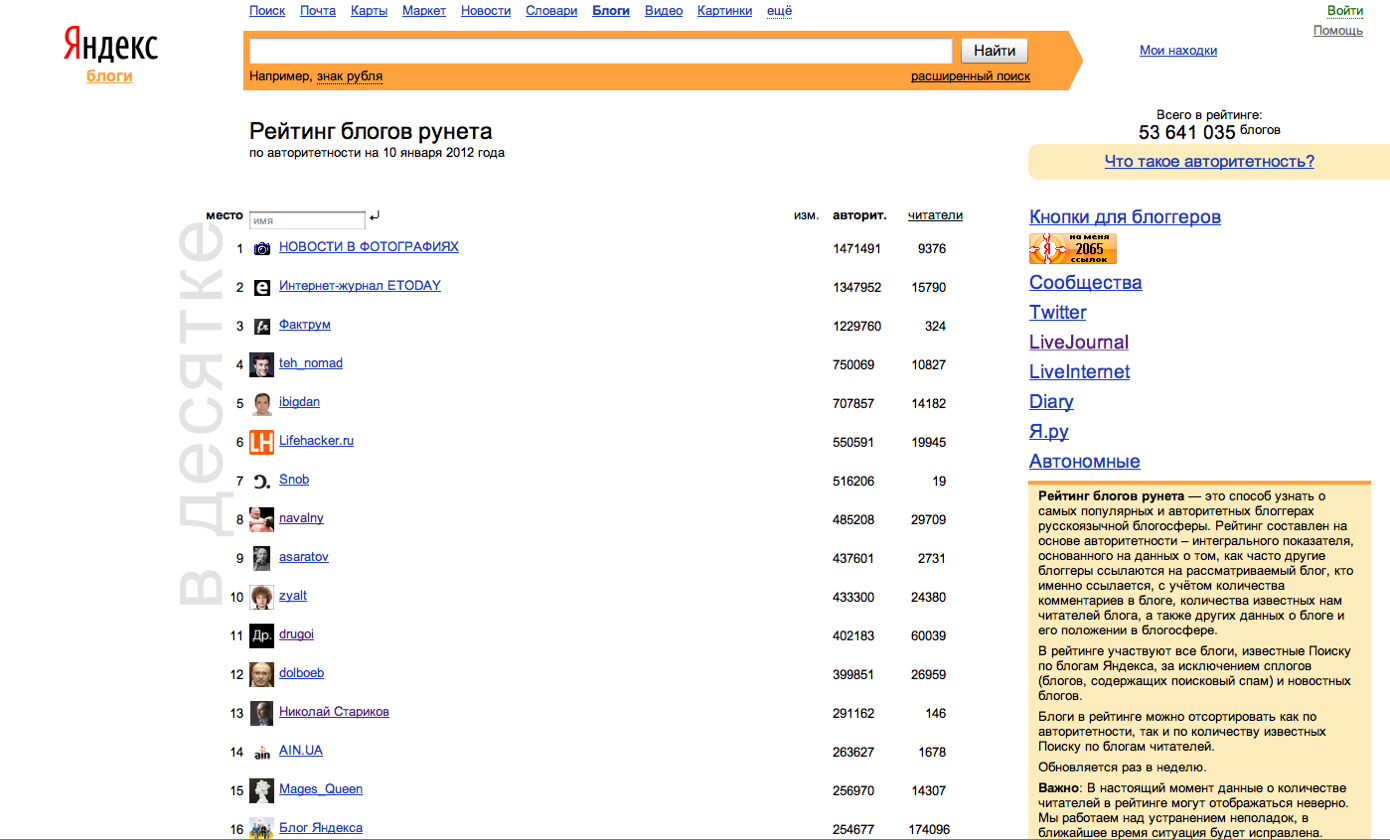
\includegraphics[width=0.9\textwidth]{images/yandex-top.png}}
\end{frame}

\section{Популяризация}
\subsection{Популяризация}
\begin{frame}
	\begin{center}
	\Huge{Как продвинуть свой блог?}
	\end{center}
\end{frame}

\subsection{Пишите интересно!}
\begin{frame}
	\begin{center}
	\huge{Пишите интересно!}
	\end{center}
	\begin{itemize}
		\item Самое важное правило!
		\item Если вы пишете интересно, читатели всегда найдутся.
		\item Не растекайтесь в мыслях. Выберите одну или несколько тем и следуйте им.
	\end{itemize}
\end{frame}

\subsection{Ищите сообщников!}
\begin{frame}
	\begin{center}
	\huge{Ищите ``сообщников''!}
	\end{center}
	\begin{itemize}
		\item Вы пишите не одни на заданную тему.
		\item Найдите других блоггеров в смежных областях.
		\item Комментируйте и ``френдуйте'' их. Кто-нибудь сделает то же самое в ответ.
		\item Не стесняйтесь цитировать и ставить гиперссылки на других людей. Они сделают точно также. Ценность Интернета --- в его гипертекстовости.
	\end{itemize}
\end{frame}

\subsection{Следуйте тренду!}
\begin{frame}
	\begin{center}
	\huge{Следуйте тренду!}
	\end{center}
	\begin{itemize}
		\item В современной блогосфере надо быть ``в теме'' !
		\item Поспевайте за новостями. 
		\item Пишите обзоры на горячие темы.
	\end{itemize}
\end{frame}

\subsection{SEO}
\begin{frame}
	\frametitle{SEO}
	\begin{itemize}
		\item SEO (англ. Search Engine Optimization) --- оптимизация под поисковые системы.
		\item Согласно Википедии: Поисковая система учитывает следующие параметры сайта при вычислении его релевантности (степени соответствия введённому запросу):
			\begin{enumerate}
				\item плотность ключевых слов (сложные алгоритмы современных поисковиков позволяют производить семантический анализ текста, чтобы отсеять поисковый спам, в котором ключевое слово встречается слишком часто).
				\item индекс цитирования сайта, зависящий от количества и авторитетности веб-ресурсов, ссылающихся на данный сайт; многими поисковиками не учитываются взаимные ссылки (друг на друга). Зачастую также важно, чтобы ссылки были с сайтов схожей тематики, что и оптимизируемый сайт.
			\end{enumerate}
	\end{itemize}
\end{frame}

\subsection{SEO}
\begin{frame}
	\frametitle{Первые шаги}
	\begin{itemize}
		\item Оцените запросы (с помощью сервиса http://wordstat.yandex.ru), по которым люди смогут попасть на ваш блог.
		\item Проверьте, соответствуют ли названия сообщений и их тексты этим запросам. Старайтесь добиваться точного соответствия.
		\item Не берите большие запросы (десятки тысяч и более показов в месяц). Большие запросы = большие деньги = мало шансов.
		\item Но помните! Блоги делаются для людей, а не для поисковых систем.
	\end{itemize}
\end{frame}

\subsection{Задания}
\begin{frame}
  \frametitle{Задания}
  \begin{itemize}
    \item Составьте семантическое ядро вашего блога (http://goo.gl/CBqz4).
		\item Подберите 10 поисковых запросов, по которым у вас есть сообщения / будут в ближайшие месяц--два.
		\item Оцените свой текущий рейтинг (авторитетность) в сервисе Яндекс.Блоги. Следите за его динамикой.
		\item Через встроенную статистику в Blogger оцените количество посетителей, пришедших с поисковых систем.
  \end{itemize}
\end{frame}

\section{References}
\subsection{References}
\begin{frame}[fragile]
  \frametitle{References}
  \begin{itemize}
    \item Все презентации доступны на http://school.smirik.ru!
    \item Вопросы, предложения, д/з: smirik@gmail.com
  \end{itemize}
\end{frame}

\end{document}